\documentclass[xetex, aspectratio=169]{beamer}
\usepackage[utf8]{inputenc}
\usepackage[T1]{fontenc}

%% Title and authors
\title{A Non-intrusive Beamer Theme Focusing on Content}
\subtitle{simple theme}
\date{\today}
\author{\underline{Adarsh}}

% Color palette 
\definecolor{AlertColor}{HTML}{DA4D45}


% two styles light and dark
% light is default
\usetheme[style=dark]{simple}

\begin{document}

\begin{frame}
\maketitle
\end{frame}

%% Toc in first frame - takes sections and not frames
%\begin{frame}{Table of contents}
%  \setbeamertemplate{section in toc}[sections numbered]
%  \tableofcontents[hideallsubsections]
%\end{frame}

%% Just for reference - it doesn't create a new slide
\section{Why a new theme?}

\begin{frame}[fragile]{Only Content Matters}
	% examples taken from Indyk's slides
	\begin{columns}
		\column{0.33\textwidth}
		{
			\begin{figure}
				
\includegraphics[scale=0.08]{img/short}
			\end{figure}
		\begin{center}
		Short and concise sentences.
		\end{center}

		}
		
		\column{0.33\textwidth}
	{
		\begin{figure}
			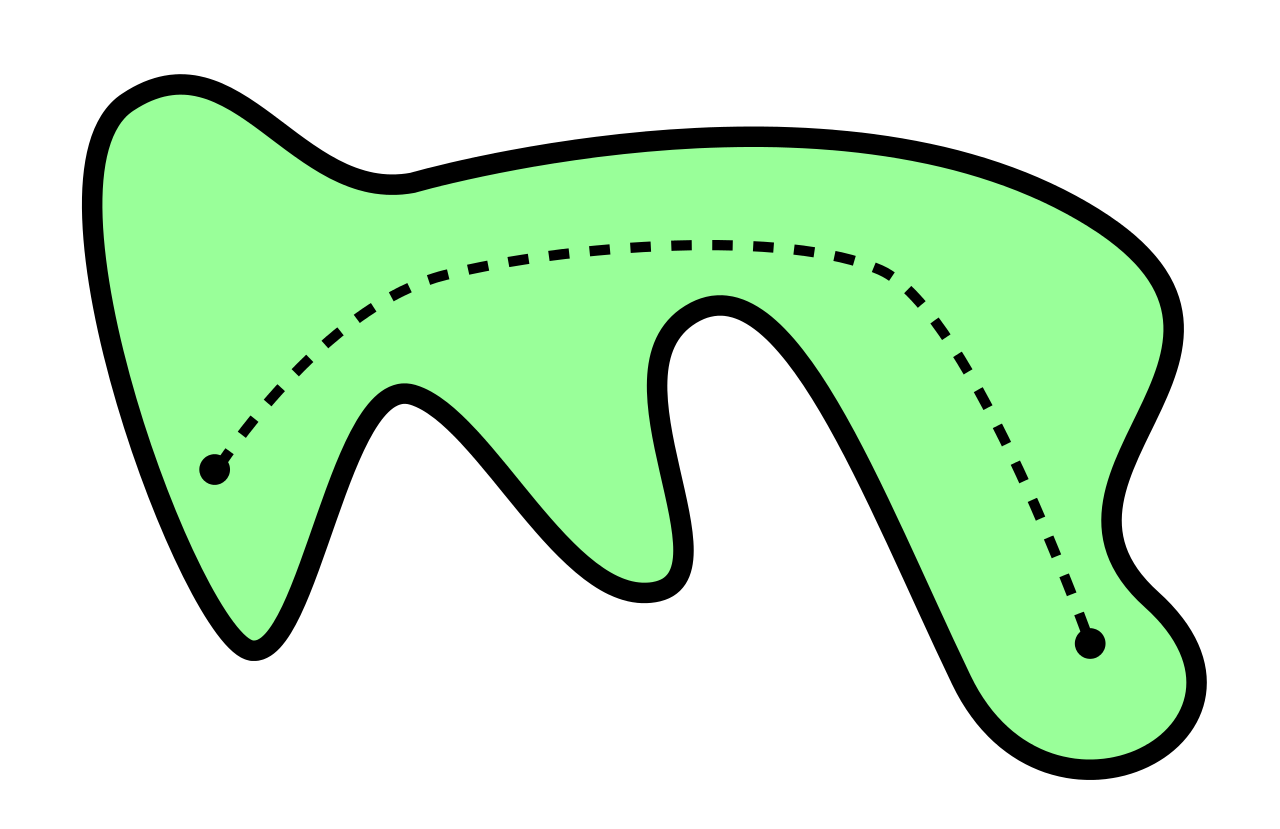
\includegraphics[scale=0.07]{img/simple}
		\end{figure}
	\begin{center}
		Simple ideas.
	\end{center}

	}
	
		\column{0.33\textwidth}
	{
		\begin{figure}
			
\includegraphics[scale=0.07]{img/smart}
		\end{figure}
	\begin{center}
		Smart presentation.
	\end{center}

	}
	
	\end{columns}
	

\end{frame}

\section{New options}

\begin{frame}[fragile]{Image with Shadow}
	

\begin{verbatim}
\shadowimage[scale=0.5]{img/visual}
\end{verbatim}

		\begin{figure}
			\shadowimage[scale=0.45]{img/visual}
			\caption{We can include images with hint of shadows}
		\end{figure}
	
\end{frame}

\begin{frame}[fragile]{Other things...}
	\begin{block}{How to use?}
Include theme in your preamble --
\begin{verbatim}
%\usetheme[style=dark]{simple}
\usetheme[style=light]{simple} 
% or  \usetheme{simple}
\end{verbatim}
	\end{block}

Equations -- 
	\begin{equation}
	A^x + B^y = ?
	\end{equation}
	
	Two styles --
	\begin{itemize}
	\item Dark Style
	\item \alert{Light Style (Default)}
	\end{itemize}
\end{frame}

\begin{frame}[fragile]{Issues}
You may have issues with font. Go to file \verb|beamerinnerthemesimple.sty| and change font to the one that you like.
\begin{verbatim}
\setsansfont{Futura Book}
\setmonofont{Monaco}
\end{verbatim}
You may comment 
\begin{verbatim}
\newfontfamily\futurabold{Futura-Bold}
\end{verbatim}
\end{frame}

\begin{frame}
	\tikz[remember picture] \node[coordinate] (n) {};
	\centering {\huge Unleash Your Creativity.... }
	\tikz[remember picture] \node[coordinate] (n1) {};
	\begin{tikzpicture}[remember picture, overlay]
	%\draw[] (-11,3) grid (3,-5);
    \node[] at (-10, 2)   (a) {What?};
    \node[] at (-9, -4)   (b) {Why?};
    \node[] at (-4, -3)   (c) {When?};
    \node[] at (-4, 2.5)   (d) {How?};
    \node[] at (2, 2)   (e) {Where?};
    \node[] at (2, -4)   (f) {Who?};
    \path[draw=AlertColor,thick,->] (a.south) to [out=-90, in=90,distance=1in] ([xshift=3cm, yshift=0.5cm]n.north);
    \path[draw=AlertColor,thick,->] (b.north) to [out=90, in=-90,distance=1in] ([xshift=3cm]n.south);
    \path[draw=AlertColor,thick,->] (c.north) to [out=90, in=-90,distance=1in] ([xshift=3.3cm]n.south);
     \path[draw=AlertColor,thick,->] (d.south) to [out=-90, in=90,distance=1in] ([xshift=3.5cm, yshift=0.5cm]n.north);
     \path[draw=AlertColor,thick,->] (e.south) to [out=-90, in=90,distance=1in] ([xshift=4cm, yshift=0.5cm]n.north);
      \path[draw=AlertColor,thick,->] (f.north) to [out=90, in=-90,distance=1in] ([xshift=4cm]n.south);
	\end{tikzpicture}
\end{frame}


\end{document}